\documentclass[11pt]{article}
\pagestyle{plain}
\usepackage{fullpage,listings,url}
\usepackage{graphicx}
\usepackage{wrapfig}
\setlength{\parindent}{0.0in}
\setlength{\parskip}{7pt plus 1pt}

\lstset{%
  	language=ruby,
	basicstyle=\scriptsize,%\ttfamily,
	frame=single,
	emph={always, once, constructor},
	emphstyle=\bfseries,
        % breaklines=true,
        breakatwhitespace=false,
        literate={<<}{$\ll$~}{1},
        showstringspaces=false,
        columns=flexible,
	}

\begin{document}

\title{Babelsberg: Integrating Constraints with an Object-Oriented Language}
\author{Tim Felgentreff and Alan Borning}
\date{Draft of \today}

\maketitle

\section{Introduction}

A constraint is a relation that we want to hold, for example, that a
resistor in an electrical circuit simulation obey Ohm's Law, that
there be a minimum of 10 pixels horizontal space between two buttons
on a screen, or that the height of a bar in a bar chart correspond to
a value produced by a simulation.  There is a long history of work on
constraint-based programming languages.  Probably the most widely
known of these is the Constraint Logic Programming scheme (ref), and
instances of this scheme such as CLP($\cal R$), which provides
constraints over the reals.  The CLP languages are in the logic
programming family, and in their standard form have no notion of state
or state change.

The most common way to to make use of constraints in an
object-oriented language, or some other sort of imperative programming
language, is via a constraint satisfaction library rather than
integrating the constraints with the language.  However, there have
been some experimental languages that attempted an actual integration
of constraints with the language.  The closest to the work described
here is the Kaleidoscope language, a constraint imperative programming
language developed in the late 1980s and early 1990s by Bjorn
Freeman-Benson, Gus Lopez, and Alan Borning (refs).  (It was the topic
of Bjorn and Gus's Ph.D. dissertations.)  Kaleidoscope was an
object-oriented language that supported standard classes and
instances.  In addition, it integrated constraints with the language
itself.  To support this, it included built-in constraints over
primitive objects (such as floats), and constraints over user-defined
objects, which were provided by \emph{constraint constructors}.  For
example, the \lstinline{+} constraint for Points could be defined
using a constraint constructor \lstinline{a+b=c} that then expanded
this into constraints on the \lstinline{x} and \lstinline{y} instance
variables of the three points \lstinline{a}, \lstinline{b}, and
\lstinline{c}.  Separately, the language also provided methods.  Both
constraint constructors and standard methods were selected using
multi-method semantics.  This accomodated, for example, the case of a
constraint constructor call \lstinline{a+b=c} in which \lstinline{b}
and \lstinline{c} were known and \lstinline{a} was unknown.

The treatment of state and time in Kaleidoscope evolved over its life.
Kaleidoscope'90 used a \emph{refinement} model, in which variables
held a stream of values, related to each other by constraints.
Variables typically had a weak stay constraint so that they retained
their value over time, e.g.\ \mbox{$x_t = x_{t-1}?$}.  (The question mark is
a read-only annotation: the constraint solver wasn't allowed to change
the past to satisfy constraints on the present.)  There were
facilities to access both the current and previous states of a
variable.  Object identity was only an implementation issue in
Kaleidoscope'90, and not semantically significant.  Later versions of
the langugage (Kaleidoscope'93) switched to a \emph{perturbation}
model, in which destructive assignment can change the state of objects
(perhaps making previously satisfied constraints unsatisfied), and the
system perturbs or adjusts values to reach a new state that best
satisfies the constraints. Instead of streams of values, a variable in
Kaleidoscope'93 referred to a single object, as in a more conventional
languages.  Kaleidoscope'93 also made object identity a part of the
language semantics, including support for identity constraints as well
as equality constraints.

Babelsberg shares many of the underlying motivations for Kaleidoscope.
However, in the twenty years since the Kaleidoscope, much has changed
with respect to the computing mileaux in which it is embedded, in
particular regarding more efficient constraint solvers, and progress
on implementation techniques for object oriented languages.

The design of Babelsberg includes a number of key decisions that we
hope will yield a more useful, practical, and performant language.
The key contributions in the language design and implementation are:

\begin{itemize}
\item a simpler semantic model (and one that is a direct extension of
  a standard object-oriented model), with ordinary methods (using
  standard object-oriented message dispatch), rather than special
  constraint constructors and multi-methods
\item for the implementation, an integration with a state of the art
  virtual machine and JIT
\end{itemize}

Additional contributions include:

\begin{itemize}
\item in the absence of constraints, the performance of a program
  written in the host language is unaffected
\item an architecture for constraint solvers that makes it
  straightforward to add new solvers, and that doesn't privilege the
  solvers provided with the basic implementation --- they are simply
  the solvers that are in the initial library
\item a solver architecture that supports multiple cooperating constraint solvers
\end{itemize}

\begin{figure} % {tb}
  \begin{center}
  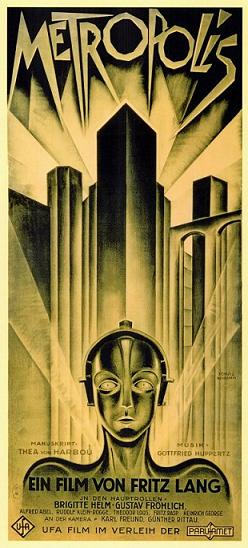
\includegraphics[width=0.25\textwidth]{Metropolisposter}
  \end{center}
\end{figure}

%% \begin{wrapfigure}{r}{0.25\textwidth}
%%   \begin{center}
%%     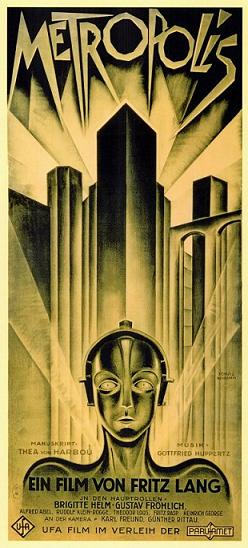
\includegraphics[width=0.25\textwidth]{Metropolisposter}
%%   \end{center}
%% \end{wrapfigure}

About the name of the language: Babelsberg is a district of Potsdam,
in which HPI is located.  It is also the location of Studio
Babelsberg, the historical center of the German film industry (Fritz
Lang's \emph{Metropolis} and Josef von Sternberg's \emph{The Blue
  Angel} were filmed there), and still active.

\section{Plan for this Note}

The plan for this note is to leave it as a draft for now, and get
comments from the Viewpoints group and others.  We then plan to submit
a journal article for the \emph{Journal of Object Technology} on the
language, based on this draft and other writings, and at the same time
publish a final version of the Viewpoints note.  The note can then be
referenced from the JOT article, and will have additional details and
a more complete description of future plans for the language.  The
target date for this is 20 July 2013.

%% For cover note to VPRI: describe relationship to CoopLangs and work
%% with Bloom.  Note that it directly used the cooperating solvers
%% architectre. 

\section{Language Design}

Babelsberg is an extension to Ruby, and Ruby programs without
constraints continue to be legal.  (The Babelsberg syntax takes
advantage of some Ruby quirks to provide a convenient syntax, and the
implementation relies on Topaz, an experimental VM built using the
PyPy/RPython toolchain.)  However, the ideas are applicable to other
dynamic object-oriented languages, and future work may include
versions in Javascript or Squeak.

\section{Implementation and Current Status}

\appendix

\section{Example Programs}

various

\bibliographystyle{plain}
\bibliography{constraints}

\end{document}
